\scanpage{93}
% archive foliation: 92
Soit $X_{\alpha\beta}=X_\alpha\cap f^{-1}(Y_\beta)$, $Y_{\beta\alpha}=Y_\beta\cap g^{-1}(X_\alpha)$, les $X_{\alpha\beta}$ et $Y_{\beta\alpha}$ sont des ens \uline{constructibles}, qui se correspondent par $f,g$.

\deleted{\unsure{Prenons} \inserted{les} $X_{\alpha\beta}$ \unsure{en une réunion finie} $\bigcup_\lambda X_{\alpha\beta\lambda}$, où $X_{\alpha\beta\lambda}$ est un sous-schéma affine constructible de $X_{\alpha\beta}$ \inserted{\unsure{et de $X_\alpha$}}. Alors $g^{-1}(X_{\alpha\beta\lambda})=g_\beta^{-1}(X_{\alpha\beta\lambda})$ est un sous-schéma de $Y_\beta$ constructible.}

\margin{\diagram{\begin{tikzcd}[ampersand replacement=\&]
X\&Y\\
\&Y_\beta\arrow[ul]
\end{tikzcd}}}

D'ailleurs $X_{\alpha\beta}=f_\alpha^{-1}(Y_\beta)$ est un \deleted{sous-schéma de} loc. fermé dans $X_\alpha$, donc dans $X$. Et $f_{\alpha\beta}:X_{\alpha\beta}\longrightarrow Y$ est un morphisme \inserted{de schémas} (car induit par $f_\alpha:X_\alpha\longrightarrow Y$]. \deleted{\unsure{Donc il est}} De même, les $Y_{\alpha\beta}$ sont constructibles et loc. fermés, et \inserted{$g_{\alpha\beta}:Y_{\alpha\beta}\longrightarrow X$ est un morphisme de schém.}

Enfin \deleted{comme} $X_{\alpha\beta}\longrightarrow Y_\beta$ se factorise par un \unsure{morph.} $X_{\alpha\beta}\longrightarrow Y_{\alpha\beta}$ [car il le fait ens.], et de même on a un \uline{morphisme} $Y_{\alpha\beta}\longrightarrow X_{\alpha\beta}$. Ces derniers sont donc inverses l'un de l'autre.

\uline{Cor. 0} Si $X$ noethérien $Y$ l'est.

\uline{Cor. 1} Tout ens schématique est isomorphe à un $|X|$, pour $X$ affine.

\uline{Cor. 2} Tout morphisme d'ens schématiques est isom. à un morphisme de \deleted{\unsure{ens}} schémas affines. (Considéré comme application constructible).

Démonstration et remarque.

\margin{\figure{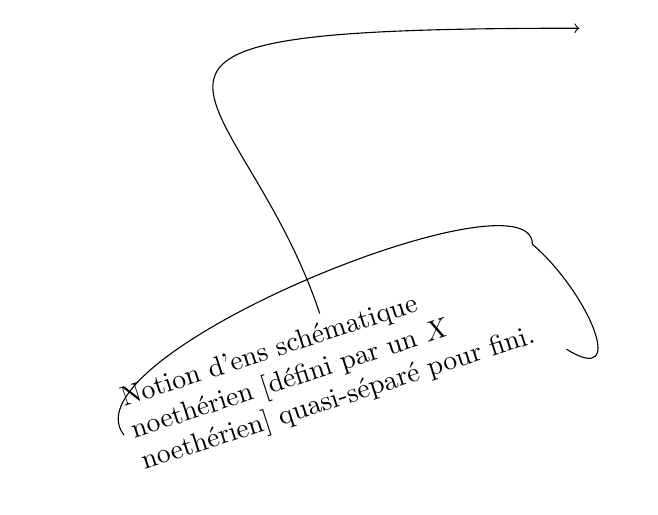
\begin{tikzpicture}
\node[anchor=north west,text width=.45\linewidth,inner sep=3pt,rotate=18] (n) at (0,0) {\uline{Notion} d'ens \unsure{schématique} \uline{noethérien} [\unsure{défini par} \unsure{un} $X$ \unsure{noethérien}] \unsure{quasi-séparé} \unsure{pour} \unsure{fini}.};
\draw[->] (n.north) .. controls +(-1,3) and +(-7,0) .. (6,4.5);
\draw (n.west) .. controls +(-.8,1) and +(0,1) .. (n.north east) .. controls +(.7,-.6) and +(.8,-.5) .. (n.south east);
\end{tikzpicture}}}

\uline{Cor. 3} Un \deleted{isom} \inserted{morphisme $f:X\longrightarrow Y$} de préschémas quasi-compacts et quasi-séparés qui est un isom d'ens schématiques est \uline{de type fini}.
% Reversed blue typewriting is transcribed on its printed face, scan 94.
